\ProvidesFile{lecture-05.tex}[Лекция 5]

\newpage

\section{Методы наискорейшего спуска и сопряженных градиентов}

\subsection*{Постановка задачи}

Рассмотрим СЛУ $Ax = y$, где $A$ --- SPD матрицей, то есть

\[
A^{\top} = A\\
\]
и
\[
\forall \, x \neq 0: x^{\top} A x > 0
\]

\begin{definition}
    \textit{Скалярным произведением} называется функция $\langle \cdot, \cdot \rangle: V \times V \longrightarrow \mathbb{R}$, где $V$ --- конечномерное векторное пространство, обладающая следующими свойствами:

    \begin{itemize}
        \item $\forall \, x, y \in V: \langle x, y \rangle = \langle y, x \rangle$

        \item $\forall \, \alpha, \beta \in \mathbb{R}, x, y, z \in V: \langle \alpha x + \beta y, z \rangle = \alpha \langle x, z \rangle + \beta \langle y, z \rangle$

        \item $\forall \, x \in V: \langle x, x \rangle > 0$
    \end{itemize}

    Иначе говоря, это симметричная положительно определенная билинейная форма
\end{definition}

\paragraph{Примеры}

\begin{itemize}
    \item Самый известный пример скалярного произведения:

    \[
    \langle x, y \rangle = x^{\top}y
    \]

    \item В общем случае скалярное произведение задается матрицей Грамма $G$ --- матрица попарных скалярных произведений базисных векторов:

    \[
    \langle x, y \rangle = \left\langle \sum\limits_{i} x_i e_i, \sum\limits_{j} y_j e_j\right\rangle = \sum\limits_{i, j} x_i y_j \langle e_i, e_j \rangle = x^{\top} G y
    \]

    \item Любая SPD матрица задает скалярное произведение:

    \[
    x^{\top} A y = \langle x, A y \rangle = \langle A x, y \rangle = \langle x, y \rangle_A
    \]
\end{itemize}

\begin{definition}
    Рассмотрим линейное векторное пространство $V$ и набор векторов $\{v_i\}_{i = 1}^n$. Тогда \textit{линейной оболочкой} будем называть подпространство $L$:

    \[
    L = \{\lambda_1 v_1 + \ldots \lambda_n v_n \mid \lambda_i \in \mathbb{R} \} = \mathrm{span}(v_1, \ldots, v_n)
    \]
\end{definition}


\begin{definition}
    При наличии скалярного произведения можно говорить об ортогональности между вектором $x \in V$ и подпространством $L$: если $\forall \, v_i \in L: \langle v_i, x \rangle = 0$. Множество векторов, которые ортогональны подпространству $L$, называется \textit{ортогональным} и обозначается как $L^{\perp}$
\end{definition}

\subsection{Метод наискорейшего спуска}

Рассмотрим следующую функцию:

\[
F(x) = \frac{1}{2} \langle x, x \rangle_A - b^{\top} x
\]

Данная функция --- квадратичная функция с положительно определенным \href{https://en.wikipedia.org/wiki/Hessian_matrix}{гессианом}, поэтому эта функция имеет единственную точку минимума. Найдем ее

\begin{itemize}
    \item Найдем производную $F'(x)$:

    \begin{multline*}
    %
    \frac{\partial F}{\partial x_k} = \frac{1}{2}\frac{\partial}{\partial x_k} \sum\limits_{i=1}^n x_i \cdot (Ax)_i - \frac{\partial}{\partial x_k} \sum\limits_{i=1}^n b_i \cdot x_i = \\
    %
    = \frac{1}{2}\frac{\partial}{\partial x_k} \sum\limits_{i=1}^n x_i \sum\limits_{j = 1}^n A_{ij} x_j - b_k = \frac{1}{2}\frac{\partial}{\partial x_k} \sum\limits_{i, j < n} x_i A_{ij} x_j - b_k = \\
    %
    = \frac{1}{2}\sum\limits_{i = 1}^n A_{ik} x_i + \frac{1}{2}\sum\limits_{i = 1}^n A_{ki} x_i - b_k = \frac{1}{2}\sum\limits_{i = 1}^n (A_{ik} + A_{ki}) x_i - b_k
    %
    \end{multline*}

    Получается, что $F'(x)$:

    \[
    F'(x) = \frac{1}{2} (A + A^{\top})x - b
    \]

    Вспомним, что $A$ --- симметрическая матрица, тогда $F'(x) = Ax - b$

    \item Получается, что задача поиска решения $Ax = b$ сводится к поиску минимума функции $F(x)$
\end{itemize}

\subsubsection*{Описание алгоритма}

\begin{itemize}
    \item Решение системы будем искать итерационно. Инициализируем стартовую точку (например, $x_1 = 0$)

    \item $k$-ую итерацию вычислим рекурсивно:
    \[
    x_{k+1} = x_k - \alpha_k r_k,
    \]

    где $r_k = b - A x_k$ --- вектор невязки (residual)

    Коэффициент $\alpha_k$ находится из минимизации функции $F(x_k + \alpha r_k)$ по $\alpha$:

    \begin{multline*}
        \frac{\partial}{\partial \alpha} F(x_k + \alpha r_k) = \frac{1}{2} \frac{\partial}{\partial \alpha} \langle x_k + \alpha r_k, x_k + \alpha r_k \rangle_A - \frac{\partial}{\partial \alpha} \langle b, x_k + \alpha r_k \rangle = \\
        %
        =\frac{1}{2} \frac{\partial}{\partial \alpha} \left(
        \langle x_k, x_k \rangle_A + \alpha^2 \langle r_k, r_k \rangle_A + 2\alpha \langle x_k, r_k \rangle_A
        \right) - \langle b, r_k \rangle = \\
        %
        = \alpha \langle r_k, r_k \rangle_A + \langle Ax, r_k \rangle - \langle n, r_k \rangle = \alpha \langle r_k, r_k \rangle_A - \langle r_k, r_k \rangle = 0 \\
    \end{multline*}

    Получаем, что

    \[
    \alpha = \frac{\langle r_k, r_k \rangle}{\langle r_k, r_k \rangle_A} = \frac{r_k^{\top} r_k}{r_k^{\top} A r_k}
    \]

    \item В итоге алгоритм имеет следующий вид:

    \begin{equation*}
        \begin{dcases*}
            x_{k+1} = x_k + \alpha_k r_k\\
            r_{k+1} = r_k - \alpha_k A r_k\\
            \alpha_k = \frac{\langle r_k, r_k \rangle}{\langle r_k, r_k \rangle_A}\\
        \end{dcases*}
    \end{equation*}
\end{itemize}

\subsubsection*{Сходимость алгоритма}

Оценим приращение функции за одну итерацию:

\[
F(x_{k+1}) - F(x_k) = \frac{1}{2}\alpha_k^2 \langle r_k, r_k \rangle_A - \alpha_k \langle r_k, r_k \rangle = [\text{подставим } \alpha_k] = -\frac{1}{2} \frac{\langle r_k, r_k \rangle^2}{\langle r_k, r_k \rangle_A}
\]

Предположим, что наш алгоритм не сходится, то есть $\lVert r_k \rVert^2 = \langle r_k, r_k \rangle_A > \varepsilon > 0$. Тогда изменение функции за один шаг можно оценить снизу константой, что означает, что за достаточное количество операций мы можем получить сколь угодно маленькое значение функции $F(x)$, что противоречит существованию минимума функции

\subsection{Метод сопряженных градинетов}

Метод наискорейшего спуска предельно прост и интуитивно понятен. К сожалению, в некоторых случаях скорость сходимости метода может быть не высока (например, когда у матрицы $A$ большее число обусловленности), так как векторы $r_k$ могут быть линейно зависимы. Эта проблема решается в следующем методе: мы будем запоминать направление на предыдущих шагах

\subsubsection*{Описание метода}

\begin{itemize}
    \item Инициализация: $x_1 = 0$ (обязательно), $r_1 = b$, $d_1 = r_1$ --- вектор направлений

    \item $k$-ая итерация:

    \begin{equation*}
        \begin{dcases*}
            x_{k+1} = x_k + \alpha_k d_k\\
            r_{k+1} = r_k - \alpha_k A d_k\\
            \alpha_k = \frac{\langle d_k, r_k \rangle}{\langle d_k, d_k \rangle_A}\\
        \end{dcases*}
    \end{equation*}

    Коэффициент $\alpha_k$ находится аналогично предыдущему методу, минимизируя $F(x_k + \alpha d_k)$ по $\alpha$.  Нетривиально вычисляется вектор $d_{k+1}$. В предыдущем методы мы всегда вдоль вектора невязки, теперь же мы смещаться вдоль ортогональной проекции вектора невязки $r_{k+1}$ на вектор направлений $d_k$

    \[
    d_{k+1} = r_{k+1} - \pr_{d_k} r_{k+1} = r_{k+1} - \frac{\langle r_{k+1}, d_k \rangle_A}{\langle d_k, d_k \rangle_A} d_k
    \]

    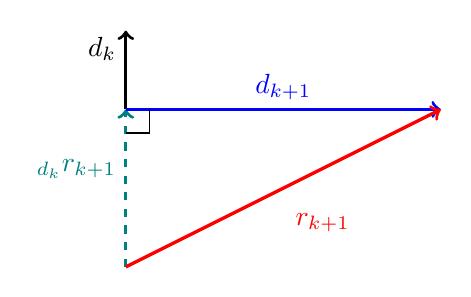
\begin{tikzpicture}
      % d_k dashed
      \draw[->, very thick, teal, dashed] (0, 0) -- (0, 2);
      % d_k
      \draw[->, very thick, black] (0, 2) -- (0, 3);

      % d_{k+1}
      \draw[->, very thick, blue] (0, 2) -- (4, 2);

      % r_{k+1}
      \draw[->, very thick, red] (0,0) -- (4, 2);

      % Right angle symbol
      \draw (0, 1.7) -- (0.3, 1.7) -- (0.3, 2);

      % Labels
      \node[above left, black] at (0, 2.5) {$d_k$};
      \node[above left, teal] at (0, 1) {$\pr_{d_k} r_{k+1}$};
      \node[above, blue] at (2, 2) {$d_{k+1}$};
      \node[below, red] at (2.5, 0.8) {$r_{k+1}$};
    \end{tikzpicture}

    \item В итоге алгоритм имеет следующий вид:

    \begin{equation*}
        \begin{dcases*}
            x_{k+1} = x_k + \alpha_k d_k\\
            r_{k+1} = r_k - \alpha_k A d_k\\
            \alpha_k = \frac{\langle d_k, r_k \rangle}{\langle d_k, r_k \rangle_A}\\
            d_{k+1} =  r_{k+1} - \frac{\langle r_{k+1}, d_k \rangle_A}{\langle d_k, d_k \rangle_A} d_k
        \end{dcases*}
    \end{equation*}
\end{itemize}

\subsubsection*{Свойства}

\begin{claim}
    Все векторы $r_k$ ортогональны между собой:

    \[
    \forall \, k_1 \neq k_2: \langle r_{k_1}, r_{k_2} \rangle = 0
    \]

    А также все $d_k$ $A$-ортогональны между собой:

    \[
    \forall \, k_1 \neq k_2: \langle d_{k_1}, d_{k_2} \rangle_A = 0
    \]
\end{claim}

\begin{proof}
    Будем доказывать по индукции по номеру итераций.

    \begin{itemize}
        \item База $k = 2$. Проверим, что $\langle r_1, r_2 \rangle = 0$ и $\langle d_1, d_2 \rangle_A = 0$.

        \[
        \langle r_1, r_2 \rangle = \left\langle r_1,
        r_1 - \frac{\langle d_1, r_1 \rangle}{\langle d_1, d_1 \rangle_A} A d_1
        \right\rangle =
        %
        \langle r_1, r_1 \rangle - \frac{\langle d_1, r_1 \rangle}{\langle d_1, d_1 \rangle_A} \langle r_1, A d_1 \rangle =
        %
        \langle r_1, r_1 \rangle - \frac{\langle r_1, r_1 \rangle}{\langle r_1, r_1 \rangle_A} \langle r_1, r_1 \rangle_A = 0
        \]

        $\langle d_1, d_2 \rangle_A = 0$ по определению.

        \item Предположение и шаг. Пусть вычислены $r_1, \ldots, r_k$ и $d_1, \ldots, d_k$ и выполнены условия ортогональности. Заметим, что

        \[
        \mathrm{span}(r_1, \ldots, r_k) = \mathrm{span}(d_1, \ldots, d_k),
        \]

        Можно доказать это равенство по индукции используя правила вычисления $r_{k+1}$ и $d_{k+1}$ в процессе алгоритма:

        \begin{equation*}
            \begin{aligned}
                &r_{k+1} = r_k - \alpha_k A d_k\\
                &d_{k+1} =  r_{k+1} - \frac{\langle r_{k+1}, d_k \rangle_A}{\langle d_k, d_k \rangle_A} d_k
           \end{aligned}
        \end{equation*}

        \begin{enumerate}
            \item Докажем ортогональность $r_k$. Вычислим $r_{k+1}$ по определению:

            \[
            r_{k+1} = r_k - \frac{\langle d_k, r_k \rangle}{\langle d_k, d_k \rangle_A} A d_k
            \]

            Поэтому вместо проверки $\langle r_{k+1}, r_i \rangle$ для $i \leqslant k$ можно проверить, что $\langle r_{k+1}, d_i \rangle$ для $i \leqslant k$. Эти утверждения равносильны. Случай $i = k$ проверяется построение. Для $i < k$:

            \[
            \langle r_{k+1}, d_i \rangle = \langle r_k, d_i \rangle - \frac{\langle d_k, r_k \rangle}{\langle d_k, d_k \rangle_A} \langle d_i, A d_i \rangle = 0 - 0 = 0 \text{ по предположению индукции}
            \]

            \item Докажем теперь $A$-ортогональность $d_k$. Случай $i = k$ проверяется построением. Для $i < k$:

            По определению $r_{i+1}$:

            \[
            r_{i+1} = r_i - \alpha_i A d_i \iff A d_i = \beta_i (r_{i+1} - r_i)
            \]

            По определению $d_{k+1}$:

            \[
            d_{k+1} = r_{k+1} - \pr_{d_k} r_{k+1} = r_{k+1} - \frac{\langle r_{k+1}, d_k \rangle_A}{\langle d_k, d_k \rangle_A} d_k
            \]

            Рассмотрим $ \langle d_i, d_{k+1} \rangle_A = \langle A d_i, d_{k+1} \rangle$:

            \begin{multline*}
                \langle A d_i, d_{k+1} \rangle = \beta_i \langle r_{i+1} - r_i, r_{k+1} \rangle - \beta_i \frac{\langle r_{k+1}, d_k \rangle_A}{\langle d_k, d_k \rangle_A} \langle r_{i+1} - r_i, d_k \rangle = \\ = \beta_i \langle r_{i+1} - r_i, r_{k+1} \rangle - \frac{\langle r_{k+1}, d_k \rangle_A}{\langle d_k, d_k \rangle_A} \langle A d_i, d_k \rangle = 0 - 0 \text{ по предположению индукции}
            \end{multline*}
        \end{enumerate}
    \end{itemize}
\end{proof}

\subsubsection*{Каноническая запись}

Найдем теперь $\langle d_k, r_k \rangle$, выразив $d_k$:

\[
\langle d_k, r_k \rangle = \langle r_k - \beta_k d_{k-1}, r_k \rangle = \langle r_k, r_k \rangle - \beta_k \langle r_k, d_{k-1} \rangle = \langle r_k, r_k \rangle - 0 = \langle r_k, r_k \rangle
\]

Так как линейные оболочки $\mathrm{span}(r_1, \ldots, r_k) = \mathrm{span}(d_1, \ldots, d_k)$ для всех $k$, то и $\langle r_k, d_{k-1} \rangle = 0$. Тогда получаем следующее:

\[
r_{k+1} = r_k - \frac{\langle r_k, r_k \rangle}{\langle d_k, d_k \rangle_A} A d_k
\]

Рассмотрим $\langle r_{k+1}, d_k \rangle_A = \langle r_{k+1}, A d_k \rangle$. Подставим $A d_k$ из выражения выше:

\[
\langle r_{k+1}, A d_k \rangle =
%
\left\langle
r_{k+1}, \frac{\langle d_k, d_k \rangle_A}{\langle r_k, r_k \rangle} \cdot (r_k - r_{k+1})
\right\rangle =
-\langle r_{k+1}, r_{k+1} \rangle \cdot  \frac{\langle d_k, d_k \rangle_A}{\langle r_k, r_k \rangle}
\]

Получаем, что

\[
d_{k+1} = r_{k+1} + \frac{\langle r_{k+1}, r_{k+1} \rangle}{\langle r_k, r_k \rangle} d_k
\]

Итоговый алгоритм на $k$-ой итерации:

\begin{equation*}
    \begin{dcases*}
        x_{k+1} = x_k + \alpha_k d_k\\
        r_{k+1} = r_k - \alpha_k A d_k\\
        \alpha_k = \frac{\langle r_k, r_k \rangle}{\langle d_k, r_k \rangle_A}\\
        \beta_k = \frac{\langle r_{k+1}, r_{k+1} \rangle}{\langle r_k, r_k \rangle}\\
        d_{k+1} = r_{k+1} + \beta_k d_k
    \end{dcases*}
\end{equation*}
